\documentclass[../delivery_hospital_report.tex]{subfiles}
\graphicspath{ {images/}{../images/}{../../images/} }
\begin{document}
\clearpage
\section{Firmware}

Cada módulo eletrônico tem o microcontrolador ESP32 \cite{esp32} para realizar o processamento de dados e comunicação com outros dispositivos embarcados, como a Jetson Nano \cite{jetson21}, o computador embarcado do Robô hospitalar. Cada microcontrolador, para realizar toda e qualquer função precisa ser devidamente programado, sem levar em consideração o circuito por trás dele, é claro. Por conta disso, cada um dos cinco módulos tem um firmware associado ao seu ESP32 específico, ou seja, cada módulo tem um código específico.

Nos primórdios do projeto, ainda na primeira versão do robô hospitalar, os códigos embarcados eram feitos em um arquivo só para cada módulo e de forma desorganizada. O maior problema disso era que isso tornava difícil compreender e adaptar os códigos. Dessa forma, há pouco mais de um mês começamos a reestruturar toda a arquitetura do firmware do projeto.

Com a nova arquitetura, os códigos associados a cada um dos módulos estão altamente relacionados com Orientação a Objeto (OO) e foram construídos com a linguagem de programação C++ \cite{c++21}, é muito recomendada para aplicações como essa, pois apresenta um baixo nível abstração, que é necessário para um firmware, e sintaxes típicas de OO. Além disso, C++ é uma linguagem que os membros da equipe do robô hospitalar já estavam familiarizados.

De maneira geral, os códigos foram feitos com base em princípios de Orientação a Objetos. Dessa forma, para cada módulo tem um único arquivo associado a ele, no qual esse arquivo utiliza uma série de bibliotecas que foram produzidas com os princípios mencionados.

\begin{figure}[!h]
\centering
    \caption{Arquitetura geral do Firmware dos módulos eletrônicos embarcados }
    \centering % para centralizarmos a figura
    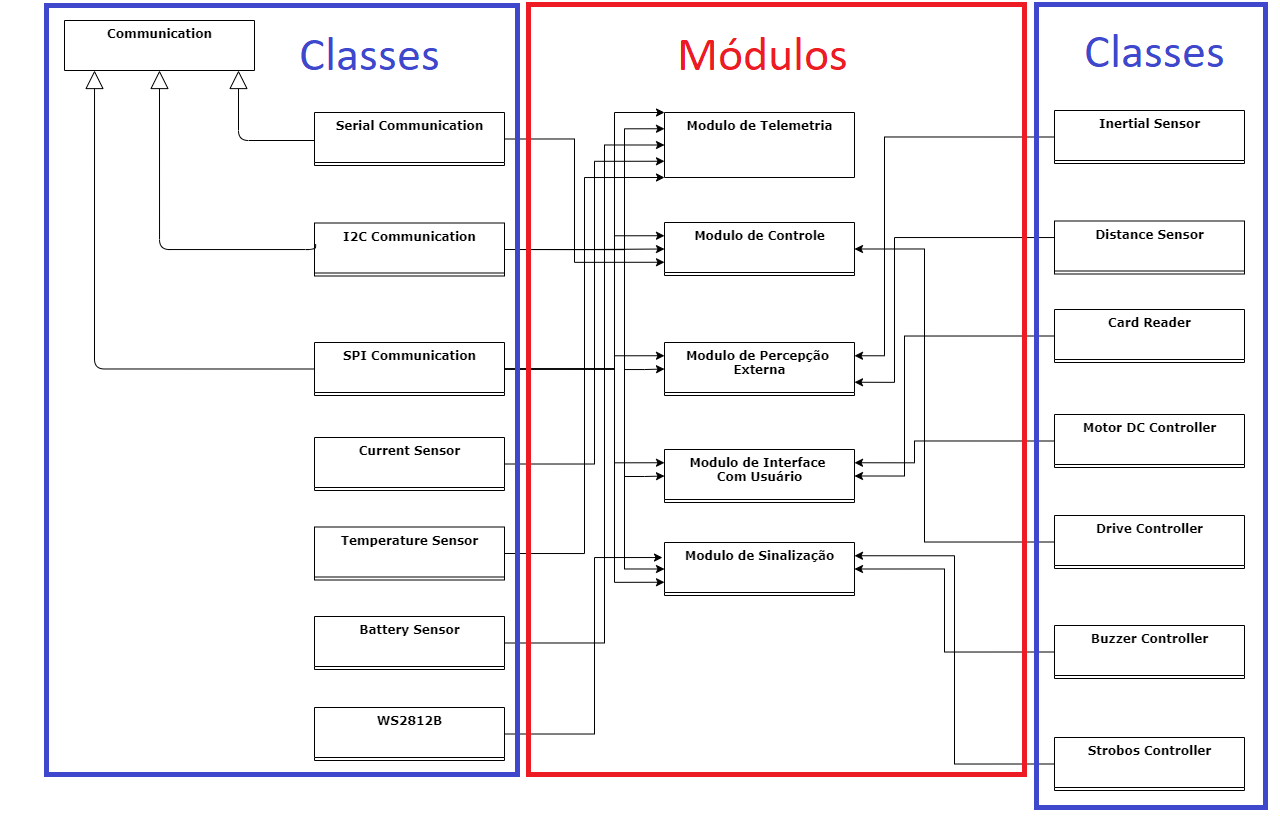
\includegraphics[width=17cm]{modulos/classes_firmware.png}
    \caption*{Fonte: Elaborado pelo autor }
    \label{Protótipo placa de ## - Esquemático principal}
\end{figure}

Por fim, essa organização mais padronizada e associada a orientação a objetos, além de permitir uma maior portabilidade e vida útil do código, ainda facilita a compreensão dos  scripts como um todo para os futuros membros do robô hospitalar.

\end{document}

